In this chapter, in \cref{exp:model_tests}, we evaluate the proposed heuristic against the MILP model (\ref{sec:milp}), and in \cref{exp:literature_tests} against other heuristics from the literature. We then show the effectiveness of our approach for our case study in \cref{exp:usecase_results}.
All the tests were run on a desktop computer with an AMD Ryzen-7 5800x processor with 8 cores at 3.8 GHz and 32GB of DDR4 system RAM with Windows 10. The algorithm was implemented in Java 11, and the model was run using the python APIs from CPLEX Optimization Studio 22.1.0.
In every test, CPLEX was used with a maximum runtime of 1 hour.
Each evaluation against the heuristic lists both operational modes described in \cref{def:placement_modes} listed as PM and PS.
All the instances used in each section of this chapter are available at \url{https://github.com/artumino/BinPackingThesis/tree/main/tests/instances}.
Out of the 100 instances used for our case study experiments, only 80 were freely sharable with the generation procedure also described in \cref{exp:usecase_results}.

\section{Model validation}
We compared our heuristic to the proposed MILP model of \cref{sec:milp} with a single bin and with no limit on the height of the bin (also referred to as the 3D strip packing problem).
The heuristic was configured to run without vertex support, using only area support rules for its feasibility checks, and $k$ was set to $200$.
The configured parameters for the test were $\alpha_s = 0.7$, $\beta_s = 5$, and the discretization unit for the model was $\delta = 10$.
Tests were run on the first generated instance of the class 1 problems from \citep{martello2000three} which we used for literature tests. These classes of problem have a bin base of $100 \times 100$.
The test were run with an iterative approach by selecting only a limited amount of items from the selected instance, starting from the first item and increasing the number of items to pack by one at each iteration.
The problem created with each iteration was saved as a test instance in the same format as the one used for literature tests.
All the generated instances are available at \url{https://github.com/artumino/BinPackingThesis/tree/main/tests/instances/model}.
A python script then loaded each generated instance sequentially and evaluated the solutions from the MILP problem and the heuristic.
Each instance was run with a time limit of 1 hour. All instances with a MIP gap lower than $4\%$ were accepted.
All instances resolved to optimality, except for instance 8, which terminated with a MIP gap of $0.02\%$.

Table \ref{exp:model} shows the obtained $z_{\text{max}}$ value of the heuristic and the MILP solution, the runtime in seconds, and the number of items.
Since the underlying problem is NP-Hard, it is shown that starting from instances of size bigger than 8 items; the MILP model becomes too slow for practical use while our heuristic maintains negligible execution time.
Due to discretization errors, some of the model instances gave solutions that didn't have the expected amount of support and were marked with an asterisk.
The solution to instance number 5 and instance number 7 is also shown in \cref{fig:model_tests}.
\label{exp:model_tests}
\begin{table}[htbp]
    \centering
    \caption{Comparison with MILP model on limited set of boxes}
    \begin{tabular}{|c|c|c|c|c|c|c|c|}
    \hline
    & \multicolumn{ 3}{c|}{\textbf{MILP Model}} & \multicolumn{ 2}{c|}{\textbf{PM}} & \multicolumn{ 2}{c|}{\textbf{PS}} \\ \hline
    \textbf{$n$} & \textbf{Max Z} & \textbf{TT(s)} & \textbf{Gap($\%$)} & \textbf{Max Z} & \textbf{TT(s)} & \textbf{Max Z} & \textbf{TT(s)} \\ \hline
    1  & 85   & 0.01     & 0.00 & 85  & 0.00 & 85  & 0.00 \\ 
    2  & 85   & 0.07     & 0.00 & 85  & 0.00 & 85  & 0.00 \\ 
    3  & 85   & 0.13     & 0.00 & 85  & 0.00 & 85  & 0.00 \\ 
    4  & 85   & 0.20     & 0.00 & 85  & 0.01 & 85  & 0.01 \\ 
    5  & 85   & 2.02     & 0.00 & 85  & 0.02 & 85  & 0.02 \\ 
    6  & 158  & 90.58    & 0.00 & 158 & 0.06 & 158 & 0.05 \\ 
    7  & 158  & 1,369.24 & 0.00 & 158 & 0.07 & 158 & 0.08 \\ 
    8  & 161* & 3,600.00 & 1.86 & 160 & 0.10 & 160 & 0.08 \\ \hline
    9  & -    & -        & -    & 169 & 0.09 & 161 & 0.10 \\ 
    10 & -    & -        & -    & 218 & 0.12 & 218 & 0.13 \\ 
    11 & -    & -        & -    & 240 & 0.12 & 240 & 0.12 \\ 
    12 & -    & -        & -    & 310 & 0.13 & 316 & 0.16 \\ 
    13 & -    & -        & -    & 310 & 0.15 & 333 & 0.18 \\ 
    14 & -    & -        & -    & 310 & 0.20 & 333 & 0.22 \\ 
    15 & -    & -        & -    & 406 & 0.21 & 397 & 0.27 \\ 
    16 & -    & -        & -    & 435 & 0.23 & 452 & 0.36 \\ 
    17 & -    & -        & -    & 429 & 0.27 & 515 & 0.41 \\ 
    18 & -    & -        & -    & 432 & 0.32 & 522 & 0.47 \\ 
    19 & -    & -        & -    & 458 & 0.35 & 522 & 0.55 \\ 
    20 & -    & -        & -    & 539 & 0.37 & 564 & 0.62 \\ \hline
    \end{tabular}
    \label{exp:model}
    \caption*{* Some boxes had lower support than expected due to discretization errors.}
    \end{table}

\begin{table}[htbp]
    \centering
    \caption{Comparison with MILP model on limited set of boxes}
    \begin{tabular}{|c|c|c|c|c|c|c|c|}
    \hline
    & \multicolumn{ 3}{c|}{\textbf{MILP Model}} & \multicolumn{ 2}{c|}{\textbf{PM}} & \multicolumn{ 2}{c|}{\textbf{PS}} \\ \hline
    \textbf{$n$} & \textbf{Max Z} & \textbf{TT(s)} & \textbf{Gap($\%$)} & \textbf{Max Z} & \textbf{TT(s)} & \textbf{Max Z} & \textbf{TT(s)} \\ \hline
    1  & 85   & 0.01     & 0.00 & 85  & 0.00 & 85  & 0.00 \\ 
    2  & 85   & 0.07     & 0.00 & 85  & 0.00 & 85  & 0.00 \\ 
    3  & 85   & 0.13     & 0.00 & 85  & 0.00 & 85  & 0.00 \\ 
    4  & 85   & 0.20     & 0.00 & 85  & 0.01 & 85  & 0.01 \\ 
    5  & 85   & 2.02     & 0.00 & 85  & 0.02 & 85  & 0.02 \\ 
    6  & 158  & 90.58    & 0.00 & 158 & 0.06 & 158 & 0.05 \\ 
    7  & 158  & 1,369.24 & 0.00 & 158 & 0.07 & 158 & 0.08 \\ 
    8  & 161* & 3,600.00 & 1.86 & 160 & 0.10 & 160 & 0.08 \\ \hline
    9  & -    & -        & -    & 169 & 0.09 & 161 & 0.10 \\ 
    10 & -    & -        & -    & 218 & 0.12 & 218 & 0.13 \\ 
    11 & -    & -        & -    & 240 & 0.12 & 240 & 0.12 \\ 
    12 & -    & -        & -    & 310 & 0.13 & 316 & 0.16 \\ 
    13 & -    & -        & -    & 310 & 0.15 & 333 & 0.18 \\ 
    14 & -    & -        & -    & 310 & 0.20 & 333 & 0.22 \\ 
    15 & -    & -        & -    & 406 & 0.21 & 397 & 0.27 \\ 
    16 & -    & -        & -    & 435 & 0.23 & 452 & 0.36 \\ 
    17 & -    & -        & -    & 429 & 0.27 & 515 & 0.41 \\ 
    18 & -    & -        & -    & 432 & 0.32 & 522 & 0.47 \\ 
    19 & -    & -        & -    & 458 & 0.35 & 522 & 0.55 \\ 
    20 & -    & -        & -    & 539 & 0.37 & 564 & 0.62 \\ \hline
    \end{tabular}
    \label{exp:model}
    \caption*{* Some boxes had lower support than expected due to discretization errors.}
    \end{table}


\clearpage
\section{Literature results}
The heuristic was also evaluated against instances from the literature defined by \citep{martello2000three}.
Since these instances were designed for heuristics without the vertical support constraint and orthogonal rotations, we ran the experiments with a relaxed version of our heuristic.
The heuristic was configured to ignore the support constraint with $\alpha_s = 0$ and $\beta_s = 1$. We also disabled orthogonal rotations and stopped scoring insertions based on the support area available (as described in \cref{ssec:scoring_insertions}).

\label{def:class1_instances}
The literature instances are divided into classes from 1 to 8, with each class having a different bin size and various distributions of types of items.
Instances were generated with the C++ instance generator provided by \citep{martello2000three} at \url{http://hjemmesider.diku.dk/~pisinger/new3dbpp/test3dbpp.c} which allows the generation of problem instances with a given problem class and number of items to use.
We generated 10 instances for each pair of problem class and number of items $n \in \{50, 100, 150, 200\}$ for a total of $320$ instances.

In \cref{exp:literature_bins} we compare the average number of opened bins across 10 instances for each problem class and $n$ number of items combinations.
The results are then compared to the most effective methods from the literature ordered by publishing date and listed as TS3 \citep{lodi2002heuristic}, GLS \citep{faroe2003guided}, GASP \citep{crainic2009ts2pack}, GVND \citep{parreno2010hybrid}, EHGH2 \citep{hifi2014hybrid}, BRKGA \citep{gonccalves2013biased}, BRKGA-VD \citep{zudio2018brkga}.
It is noted that values for other heuristics are reported as in their publications, and our generated instances weren't the same ones which, as indicated in \citep{hifi2014hybrid}, could have different optimal values.
The best values of all the heuristics are marked in bold. Best scoring values across different configurations of our heuristic are marked in italic instead.
Results show an average gap of $4.1\%$ compared to the average value across the other heuristics and an average gap of $5.32\%$ with respect to the best performing one.

In \cref{exp:literature_time_gap} we give an approximate comparison between the average execution time of our heuristic with respect to BRKGA-VD.
Execution times for BRKGA-VD were normalized by comparing directly the floating-point operations per second of the processors used, which resulted in dividing BRKGA-VD execution times by a normalization term of $9.3$. %FIXME: Remove this and use unscaled times, specify computer for BRKGA
The values presented are the times averaged across 8 classes of problems divided according to the size of the instance and the heuristic configuration. In the last column, we also included the average gap of each configuration of the heuristic with respect to the values of BRKGA-VD.
\label{exp:literature_tests}
\begin{table}[htbp]
    \centering
    \caption{Literature results for $k=50$}
    \resizebox{\textwidth}{!}{\begin{adjustbox}{angle=90}
    \begin{tabular}{|c|c|c|c|c|c|c|c|c|c|c|}
    \hline
    \textbf{Class} & \textbf{n} & \textbf{PM} & \textbf{PS} & \textbf{TS3} & \textbf{GLS} & \textbf{GASP} & \textbf{EHGH2} & \textbf{GVN} & \textbf{BRKGA} & \textbf{BRKGA-VD} \\ 
    & & $k=50$ & $k=50$ &  &  &  &  &  &  &  \\ \cline{ 3- 11}\hline
    1 & 50 & 14.10 & \textit{14} & \textbf{13.4} & \textbf{13.4} & \textbf{13.4} & 13.8 & \textbf{13.4} & \textbf{13.4} & \textbf{13.4} \\ 
     & 100 & 28 & \textit{27.7} & \textbf{26.6} & \textbf{26.6} & 26.9 & 27.6 & \textbf{26.6} & \textbf{26.6} & \textbf{26.6} \\ 
     & 150 & 38.4 & \textit{37.9} & 36.7 & 37 & 37 & 39.8 & 36.4 & 36.4 & \textbf{36.3} \\ 
     & 200 & 53 & 52.7 & 51.2 & 51.2 & 51.6 & \textbf{50.6} & 50.9 & 50.8 & 50.8 \\ \hline
    2 & 50 & \textit{14.6} & 14.8 & \textbf{13.8} & - & - & - & \textbf{13.8} & \textbf{13.8} & \textbf{13.8} \\ 
     & 100 & 26.6 & 26.7 & 25.7 & - & - & - & 25.7 & 25.6 & \textbf{25.5} \\ 
     & 150 & 38.3 & 39 & 37.2 & - & - & - & 36.9 & \textbf{36.6} & \textbf{36.6} \\ 
     & 200 & \textit{51} & 51.7 & 50.1 & - & - & - & \textbf{49.4} & \textbf{49.4} & \textbf{49.4} \\ \hline
    3 & 50 & 13.9 & 13.9 & \textbf{13.3} & - & - & - & \textbf{13.3} & \textbf{13.3} & \textbf{13.3} \\ 
     & 100 & 27.8 & 27.3 & 26 & - & - & - & 26 & \textbf{25.9} & \textbf{25.9} \\ 
     & 150 & 39.2 & 39 & 37.7 & - & - & - & 37.6 & \textbf{37.5} & \textbf{37.5} \\ 
     & 200 & 51.8 & \textit{51.2} & 50.5 & - & - & - & 50 & \textbf{49.8} & \textbf{49.8} \\ \hline
    4 & 50 & \textit{29.7} & \textit{29.7} & \textbf{29.4} & \textbf{29.4} & \textbf{29.4} & \textbf{29.4} & \textbf{29.4} & \textbf{29.4} & \textbf{29.4} \\ 
     & 100 & \textit{59.2} & \textit{59.2} & 59 & 59 & 59 & 59.5 & 59 & 59 & \textbf{58.9} \\ 
     & 150 & \textit{87.6} & 87.7 & \textbf{86.8} & \textbf{86.8} & \textbf{86.8} & 90.4 & \textbf{86.8} & \textbf{86.8} & \textbf{86.8} \\ 
     & 200 & \textit{119.5} & \textit{119.5} & \textbf{118.8} & 119 & \textbf{118.8} & 119 & \textbf{118.8} & \textbf{118.8} & \textbf{118.8} \\ \hline
    5 & 50 & \textit{8.6} & \textit{8.6} & 8.4 & 8.3 & 8.4 & \textbf{7.9} & 8.3 & 8.3 & 8.3 \\ 
     & 100 & 16 & \textit{15.6} & 15 & 15.1 & 15.1 & \textbf{14.6} & 15 & 15 & 15 \\ 
     & 150 & 21.7 & 21.4 & 20.4 & 20.2 & 20.6 & 21.5 & 20.4 & 20.1 & \textbf{19.9} \\ 
     & 200 & 29 & 28.4 & 27.6 & 27.2 & 27.7 & 29.6 & \textbf{27.1} & \textbf{27.1} & \textbf{27.1} \\ \hline
    6 & 50 & \textit{10} & 10.3 & 9.9 & 9.8 & 9.9 & 11.8 & 9.8 & \textbf{9.7} & \textbf{9.7} \\ 
     & 100 & 19.8 & 19.7 & 19.1 & 19.1 & 19.1 & 19.2 & 19 & \textbf{18.9} & \textbf{18.9} \\ 
     & 150 & 30.3 & 30.2 & 29.4 & 29.4 & 29.5 & 29.8 & 29.2 & \textbf{29} & \textbf{29} \\ 
     & 200 & 38.9 & \textit{38.5} & 37.7 & 37.7 & 38 & 38.7 & 37.4 & \textbf{37.3} & \textbf{37.3} \\ \hline
    7 & 50 & 7.8 & \textit{7.6} & 7.5 & \textbf{7.4} & 7.5 & \textbf{7.4} & \textbf{7.4} & \textbf{7.4} & \textbf{7.4} \\ 
     & 100 & \textit{13.2} & \textit{13.2} & 12.5 & 12.3 & 12.7 & 13.5 & 12.5 & \textbf{12.2} & \textbf{12.2} \\ 
     & 150 & 17.1 & 16.8 & 16.1 & 15.8 & 16.6 & 18.2 & 16 & 15.3 & \textbf{15.2} \\ 
     & 200 & 24.9 & 24.7 & 23.9 & 23.5 & 24.2 & 24.1 & 23.5 & \textbf{23.4} & \textbf{23.4} \\ \hline
    8 & 50 & 9.9 & 9.7 & 9.3 & \textbf{9.2} & 9.3 & 9.4 & \textbf{9.2} & \textbf{9.2} & \textbf{9.2} \\ 
     & 100 & \textit{19.6} & 20 & 18.9 & 18.9 & 19 & 18.9 & 18.9 & 18.9 & \textbf{18.8} \\ 
     & 150 & 25.7 & 25.8 & 24.1 & 23.9 & 24.8 & 26 & 24.1 & \textbf{23.6} & \textbf{23.6} \\ 
     & 200 & 31.6 & \textit{31.2} & 30.3 & 29.9 & 31.1 & 35.8 & 29.8 & \textbf{29.3} & \textbf{29.3} \\ \hline
    \end{tabular}
    \end{adjustbox}}
    \label{exp:literature_bins}
    \end{table}
    
\begin{table}[htbp]
    \caption{Average execution time of literature results with bin gap}
    \centering
    \resizebox{\textwidth}{!}{\begin{tabular}{|l|l|c|c|c|c|c|}
    \hline
    \multicolumn{2}{|c|}{\textbf{Heuristic}} & \multicolumn{4}{|c|}{\textbf{Execution Time (s)}} & \textbf{Bin Gap (\%)} \\ \hline
    \multicolumn{2}{|c|}{} & $n=50$ & $n=100$ & $n=150$ & $n=200$ &  \\ \hline
    \textbf{PM} & $k=1$ & 0.03 & 0.11 & 0.28 & 0.54 & 5.82 \\ 
     & $k=5$ & 0.08 & 0.38 & 1.00 & 2.09 & 5.56 \\ 
     & $k=10$ & 0.15 & 0.73 & 1.93 & 4.00 & 5.54 \\ 
     & $k=20$ & 0.29 & 1.40 & 3.77 & 7.71 & 5.30 \\ 
     & $k=50$ & 0.70 & 3.50 & 9.39 & 19.59 & 5.19 \\ \hline
    \textbf{PS} & $k=1$ & 0.05 & 0.18 & 0.50 & 1.05 & 5.61 \\ 
     & $k=5$ & 0.12 & 0.72 & 2.10 & 4.62 & 5.26 \\ 
     & $k=10$ & 0.23 & 1.38 & 4.11 & 8.95 & 5.19 \\ 
     & $k=20$ & 0.46 & 2.67 & 8.21 & 17.64 & 4.98 \\ 
     & $k=50$ & 1.12 & 6.45 & 20.39 & 43.50 & 4.75 \\ \hline
     \hline
     \multicolumn{2}{|l|}{\textbf{BRKGA-VD}} & 17.13 & 80.63 & 190.50 & 369.75 & 0.00 \\ \hline
    \end{tabular}}
    \label{exp:literature_time_gap}
\end{table}
    

\clearpage
\section{Case study results}
Case study experiments were conducted on a series of problem instances that were divided between 20 real-world instances and 80 generated instances composed of items sampled from a population of real-world products.
Each instance was anonymized and converted to a format similar to the one used for the literature tests thanks to a Rust program available at \url{https://github.com/artumino/BinPackingThesis/tree/main/additional/testConverter}.
Support parameters for the heuristic were set to $\alpha_s = 0.7$ and $\beta_s = 10$ with both area and vertex support enabled. All dimensions of the bin, items, and tolerances are assumed to be in millimeters.
Different values of $k \in \{1, 5, 10, 20, 50, 100, 200\}$ were tested as well as both placement modes.

Each generated instance is composed of a random number of $n$ items sampled from a given range of possible instance sizes. All generated instances had a bin of standard size $800 \times 1200 \times 2000$.
We identified four ranges of interest and generated 20 instances for each range as follows:
\begin{itemize}
    \item \textbf{Class 1-20}: a class of instances with the target sizes for our case-study $n \in [70,100]$
    \item \textbf{Class 21-40}: a class of small sized instances with number of items $n \in [50,70]$
    \item \textbf{Class 41-60}: a class of medium sized instances with number of items $n \in [70,120]$
    \item \textbf{Class 61-80}: a class of big instances with number of items $n \in [120,200]$
\end{itemize}

Given an input $n$ (the size of the test instance), the generation procedure uniformly sampled an item type from a population of real-world products.
The quantity of items of that type to add to the test instance was then sampled from a normal distribution $\mathcal{N}(\mu = 4.6, \sigma = 1.8)$ with parameters calculated from the real-world instances.
The sampled quantity was then floored to be an integer value and clamped to avoid generating more items than $n$.
This uniform sampling of item types was done until the instance was composed of $n$ items.

Real-world instances are listed as \textbf{Class 81-100} and have a variable number of items between $[25, 345]$, a variable bin size (although similar to the one used for the generated instances), and a variable number of items of the same type. Some instances were homogeneous with only a few unique items, and some were heterogeneous with every item of a different type.
An example of real-world instances is shown in \cref{fig:usecase_tests} where items of the same shape are marked with the same color.

Table \ref{exp:usecase_results} shows the average results over the 20 instances per class, divided by each configuration of the heuristic with different values of $k$.
The results shown include the total execution time in milliseconds (TT), the number of opened bins (B), and the average cage ratio between the opened bins (CR).
It is clear that although the PS method had better results when dealing with a relaxed version of the problem, grouping items by type shows considerable improvements under all measured metrics when taking vertical support into account.
Most of the configurations lead to an average cage ratio of more than $70\%$, which was the target value for our case study. %FIXME: rephrase this to address the previous solution for our clients which was 60% CR on average
It is also possible to see that increasing the value of $k$ improves the quality of the solutions, on average, at the expense of a higher execution time.
By doing a case-by-case analysis of each experiment, we discovered that increasing $k$ can temporarily worsen the solution in some instances.
A further study of the problematic instances highlighted that the current greedy scoring mechanism of the states leads to cutting out good solutions too early. %FIXME: more explaining, count better ks
Further improvements are proposed in \cref{chapther:conclusions}.
\label{exp:usecase_results}
\begin{table}[htbp]
    \centering
    \caption{Summary of use-case tests}
    \begin{tabular}{|l|l|c|c|c|c|c|c|}
    \hline
    \multicolumn{ 2}{|c|}{\textbf{Instance}} & \multicolumn{ 3}{c|}{\textbf{Single Placement}} & \multicolumn{ 3}{c|}{\textbf{Order by Hash}} \\ \hline
    \multicolumn{ 2}{|l|}{} & \textbf{\textit{TT (ms)}} & \textbf{\textit{B}} & \textbf{\textit{CR}} & \textbf{\textit{TT (ms)}} & \textbf{\textit{B}} & \textbf{\textit{CR}} \\ \hline
    \multicolumn{1}{|r|}{\textbf{Global}} & k=1 & 423.87 & 1.37 & 65.87 & 65.18 & 1.31 & \textbf{70.70} \\ 
     & k=5 & 1,597.54 & 1.34 & 69.19 & 185.22 & 1.29 & \textbf{73.08} \\ 
     & k=10 & 2,627.52 & 1.32 & 70.35 & 344.90 & 1.27 & \textbf{73.56} \\ 
     & k=20 & 5,373.79 & 1.34 & 70.78 & 620.95 & 1.27 & \textbf{74.57} \\ 
     & k=50 & 14,203.10 & 1.31 & 72.11 & 1,279.96 & 1.29 & \textbf{74.61} \\ 
     & k=100 & 26,934.21 & 1.31 & 73.23 & 2,340.37 & 1.26 & \textbf{75.36} \\ 
     & k=200 & 48,944.90 & 1.30 & 73.89 & 4,465.78 & 1.25 & \textbf{76.39} \\ \hline
    \multicolumn{1}{|r|}{\textbf{Class 1-20}} & k=1 & 187.25 & 1.15 & 64.10 & 54.95 & 1.05 & \textbf{70.69} \\ 
     & k=5 & 489.40 & 1.05 & 70.38 & 111.75 & 1.00 & \textbf{75.36} \\ 
     & k=10 & 861.30 & 1.05 & 71.94 & 182.20 & 1.00 & \textbf{75.77} \\ 
     & k=20 & 1,588.15 & 1.05 & 72.04 & 308.45 & 1.00 & \textbf{76.60} \\ 
     & k=50 & 3,896.40 & 1.05 & 73.07 & 690.80 & 1.00 & \textbf{76.95} \\ 
     & k=100 & 7,789.90 & 1.00 & 75.45 & 1,204.35 & 1.00 & \textbf{78.46} \\ 
     & k=200 & 15,817.20 & 1.05 & 74.99 & 2,192.75 & 1.00 & \textbf{78.27} \\ \hline
    \multicolumn{1}{|r|}{\textbf{Class 21-40}} & k=1 & 50.90 & 1.00 & 68.21 & 17.80 & 1.00 & \textbf{73.66} \\ 
    \multicolumn{1}{|c|}{N = [50, 70]} & k=5 & 138.40 & 1.00 & 71.92 & 39.20 & 1.00 & \textbf{74.78} \\ 
     & k=10 & 253.10 & 1.00 & 73.15 & 74.95 & 1.00 & \textbf{75.28} \\ 
     & k=20 & 483.85 & 1.00 & 73.86 & 124.30 & 1.00 & \textbf{76.46} \\ 
     & k=50 & 1,193.55 & 1.00 & 74.77 & 288.50 & 1.00 & \textbf{77.02} \\ 
     & k=100 & 2,358.50 & 1.00 & 75.08 & 535.30 & 1.00 & \textbf{77.11} \\ 
     & k=200 & 4,769.85 & 1.00 & 76.69 & 1,033.00 & 1.00 & \textbf{78.64} \\ \hline
    \multicolumn{1}{|r|}{\textbf{Class 41-60}} & k=1 & 292.35 & 1.30 & 65.62 & 60.55 & 1.25 & \textbf{71.34} \\ 
    \multicolumn{1}{|c|}{N = [70, 120]} & k=5 & 1,025.65 & 1.30 & 67.97 & 172.35 & 1.30 & \textbf{72.53} \\ 
     & k=10 & 1,910.60 & 1.30 & 68.46 & 304.25 & 1.25 & \textbf{72.04} \\ 
     & k=20 & 3,666.40 & 1.30 & 68.68 & 571.90 & 1.25 & \textbf{74.01} \\ 
     & k=50 & 7,649.95 & 1.25 & 71.32 & 1,152.40 & 1.25 & \textbf{75.25} \\ 
     & k=100 & 15,848.15 & 1.25 & 72.90 & 1,956.55 & 1.20 & \textbf{75.67} \\ 
     & k=200 & 32,420.40 & 1.25 & 73.29 & 3,472.50 & 1.20 & \textbf{76.10} \\ \hline
    \multicolumn{1}{|r|}{\textbf{Class 61-80}} & k=1 & 1,371.00 & 2.20 & 64.68 & 158.00 & 2.05 & \textbf{69.11} \\ 
    \multicolumn{1}{|c|}{N = [120, 200]} & k=5 & 5,751.95 & 2.15 & 66.66 & 531.80 & 1.95 & \textbf{71.31} \\ 
     & k=10 & 9,040.85 & 2.05 & 68.56 & 1,033.15 & 1.90 & \textbf{72.69} \\ 
     & k=20 & 19,116.60 & 2.15 & 67.81 & 1,881.70 & 1.90 & \textbf{73.84} \\ 
     & k=50 & 52,937.40 & 2.05 & 69.94 & 3,744.70 & 2.00 & \textbf{71.25} \\ 
     & k=100 & 98,271.55 & 2.10 & 70.04 & 7,010.65 & 1.90 & \textbf{73.80} \\ 
     & k=200 & 170,191.55 & 2.00 & 71.15 & 13,544.15 & 1.90 & \textbf{75.01} \\ \hline
    \multicolumn{1}{|r|}{\textbf{Class 81-100}} & k=1 & 217.85 & 1.20 & 66.74 & 34.60 & 1.20 & \textbf{68.68} \\ 
     & k=5 & 582.30 & 1.20 & 69.03 & 71.00 & 1.20 & \textbf{71.41} \\ 
     & k=10 & 1,071.75 & 1.20 & 69.65 & 129.95 & 1.20 & \textbf{72.00} \\ 
     & k=20 & 2,013.95 & 1.20 & 71.52 & 218.40 & 1.20 & \textbf{71.97} \\ 
     & k=50 & 5,338.20 & 1.20 & 71.44 & 523.40 & 1.20 & \textbf{72.57} \\ 
     & k=100 & 10,402.95 & 1.20 & \textbf{72.68} & 995.00 & 1.20 & 71.74 \\ 
     & k=200 & 21,525.50 & 1.20 & 73.30 & 2,086.50 & 1.15 & \textbf{73.95} \\ \hline
    \end{tabular}
    \label{results:usecase_summary}
    \end{table}
    
\begin{figure}
    \centering
    \subfloat[Instance 95]{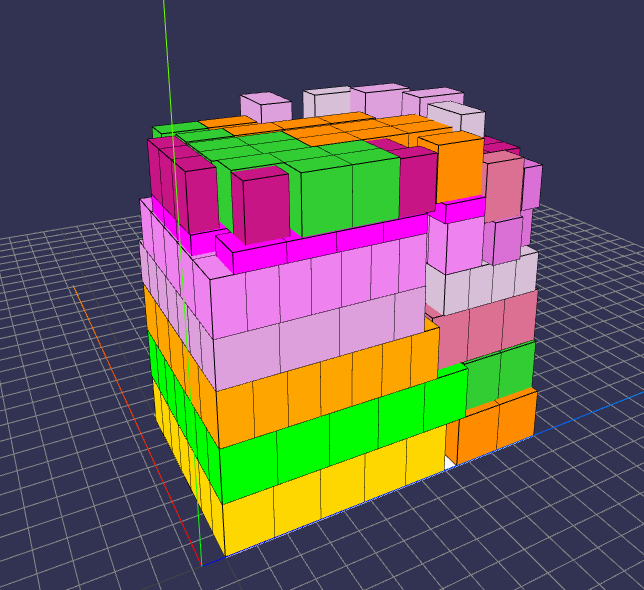
\includegraphics[width = 3in]{tests/usecase/instance-95_k200.PNG}} 
    \subfloat[Instance 82]{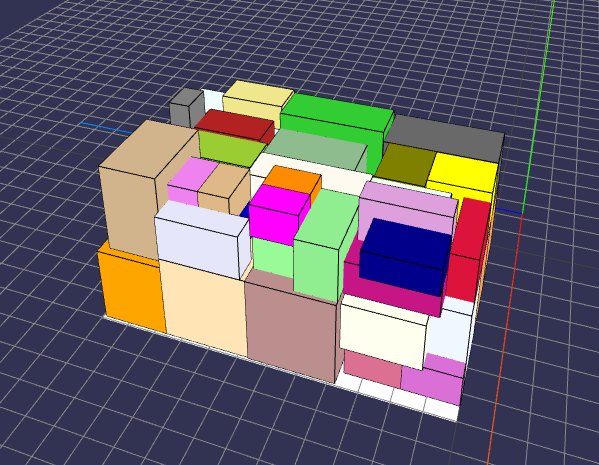
\includegraphics[width = 3in]{tests/usecase/instance-82_k200.PNG}}\\
    \subfloat[Instance 56]{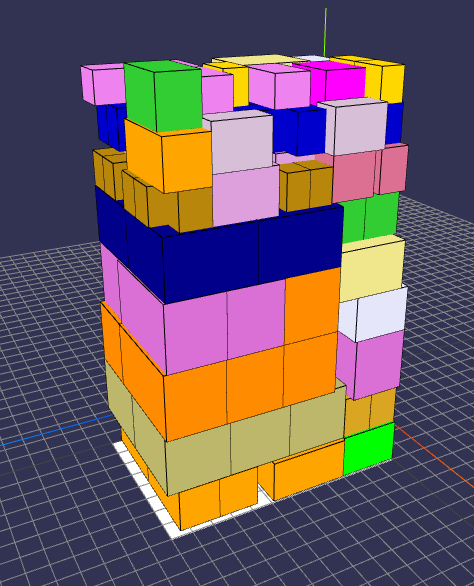
\includegraphics[width = 3in]{tests/usecase/instance-56_k200.PNG}} 
    \subfloat[Instance 66, Bin 1]{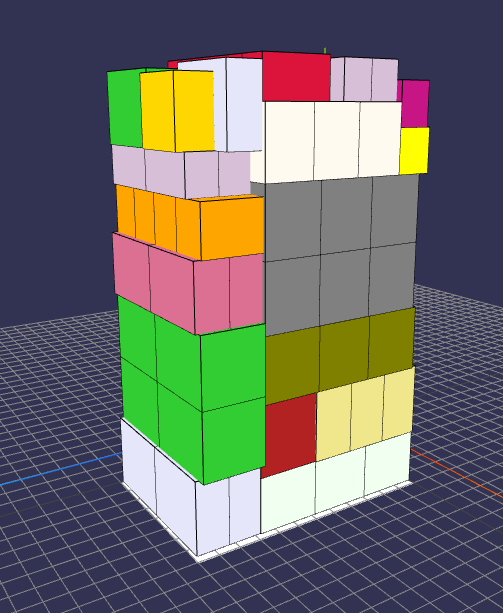
\includegraphics[width = 3in]{tests/usecase/instance-66_bin1_k200.PNG}}
    \caption{Some solutions of the use-case tests with the "Group by Hash" behaviour and $k=200$}
    \label{fig:usecase_tests}
\end{figure}